\chapter{Analysis}
\label{chapter:hps:analysis}

The design of \ac{hps} separates reconstructed tracks into categories that are
not necessarily associated with the underlying physics for which we are searching.
Specifically, the number of layers (and which layers) that are included within a track
has a large effect on the resulting precision of the reconstructed physics variables
of that track; thus, we categorize vertices on whether one or both of their tracks contain
both sensors in the first layer.
\cref{fig:hps-reco-category-diagram} shows examples of the two categories considered
within this work.
The L1L1 category whose verticies have both tracks with good precision was first studied
for this signal search \todo[citation]{need Alic's thesis} when optimizing the pre-selection
requirements described earlier.

Extending this search to the L1L2 category has a rather simple motivation.
While the vertices may degrade in precision, the additional increase of data both in terms
of total volume and the potential to observe higher-displaced vertices is expected to improve
the sensitivity of the \ac{hps} \ac{simp} search.

\begin{figure}
  \centering
  \begin{subfigure}{0.48\textwidth}
    \centering
    \resizebox{\textwidth}{!}{\begin{tikzpicture}
  \drawhpsfirsttwolayers
  \node at (\targetx,+2) {L1L1};
  \node at (\targetx+1,0.1) [circle,fill,inner sep=1.5pt] {};
  \draw[black,->] (\targetx+1,0.1) -- (2.5,2) node[anchor=north west] {\(e^-\)};
  \draw[black,->] (\targetx+1,0.1) -- (2.5,-1.9) node[anchor=south west] {\(e^+\)};
\end{tikzpicture}
}
  \end{subfigure}
  ~
  \begin{subfigure}{0.48\textwidth}
    \centering
    \resizebox{\textwidth}{!}{\begin{tikzpicture}
  \drawhpsfirsttwolayers
  \node at (\targetx,+2) {L1L2};
  \node at (\targetx+2.0,0.1) [circle,fill,inner sep=1.5pt] {};
  \draw[black,->] (\targetx+2.0,0.1) -- (2.5,2) node[anchor=north west] {\(e^-\)};
  \draw[black,->] (\targetx+2.0,0.1) -- (2.5,-1.8) node[anchor=south west] {\(e^+\)};
\end{tikzpicture}
}
  \end{subfigure}
  \caption{Diagrams showing L1L1 (left) and L1L2 (right) vertex examples.}
  \label{fig:hps-reco-category-diagram}
\end{figure}

\section{Physics Variables}
There are many possible variables that could be used to separate candidate signal
vertices from the standard process backgrounds.
While this section is not an exhaustive list of all possible variables,
it does explain the ones used within this analysis as well as motivation for
their use.

The \ac{simp} signal vertex will have significantly less energy than the amount
delivered by the beam because of the production of a light dark meson when the heavier
vector meson $V_D$ is produced.
Thus, a selection on the sum of the momentum magnitudes is applied.
\begin{equation}
  P_\mathrm{sum} = |\vec{p}_{e^-}|+|\vec{p}_{e^+}|
\end{equation}
$P_\mathrm{sum}$ is chosen to lie within the same ranges as the L1L1 analysis.
Specifically, the Signal Region (SR) used for the actual search requires
$\qty{1.0}{\GeV} < P_\mathrm{sum} < \qty{1.9}{\GeV}$ and the Control Region (CR)
used for determining the trident differential production rate is
$\qty{1.9}{\GeV} < P_\mathrm{sum} < \qty{2.4}{\GeV}$.

Since we are searching for the dark vector boson $V_D$ via its
2-body decay into an electron and a positron, we expect the invariant mass of the vertex $m_\text{reco}$
to be within the resolution of the detector $\sigma_m$ of the mass we are searching for $m_{V_D}$.
\begin{equation}
  p_m = \frac{|m_\text{reco}-m_{V_D}|}{\sigma_m}
\end{equation}
Applying an upper limit on $p_m$ is often refered to as a ``mass window''
since it results in $m_\text{reco}$ residing within a small range around $m_{V_D}$.
For the exclusion estimate and the optimization studies described in this
section, we choose $p_m < 2.8$ to align with the L1L1 analysis.

Each vertex can be projected back to the target using its position and total momentum,
and the location of the vertex at the target can be compared to the beam
position extracted from a sub-sample of the data (\todo{reference how this is done}).
The separation between the projected position $\vec{x} = (x,y)$ and the beam position
$\vec{\mu} = (\mu_{x'}, \mu_{y'})$ is then measured
and normalized by the width of the beam in that direction
$(\sigma_{x'},\sigma_{y'})$.
The distribution of the beamspot is allowed to be rotated relative to our
chosen axes by the angle $\theta_\mathrm{beam}$, meaning we need to rotate $\vec{x}$
before comparing it to the beam spot.
The total ``elliptical'' separation between the reconstructed vertex
projected back to the target and the beam spot can be quantified by
\begin{equation}
  N_\sigma = \sqrt{
    \left(
      \frac{x\cos\theta_\mathrm{beam} - y\sin\theta_\mathrm{beam} - \mu_{x'}}{\sigma_{x'}}
    \right)^2
    +\left(
      \frac{x\sin\theta_\mathrm{beam} + y\cos\theta_\mathrm{beam} - \mu_{y'}}{\sigma_{y'}}
    \right)^2
  }
\end{equation}
I refer to this as \ac{vps} since it represents how significantly
a vertex deviates from originating at the beam spot.

Since the detector's tracking modules are oriented to be most senstive in the
vertical direction, the vertical impact parameter $y_0$ has higher precision compared
to the horizontal impact parameter.
For truly-displaced signal vertices, both tracks making the vertex would have
$y_0$ far from zero while background vertices would have at least one track
with $y_0$ near zero (undisplaced vertices would have both, but mis-reconstructed
fake-displaced vertices could have one far from zero).
This motivates selecting vertices based on requiring the minimum of the two
absolute value $y_0$ to be above a certain threshold.
\begin{equation}
  y_{0,\min} = \min(|y_{0,e^-}|,|y_{0,e^+}|)
\end{equation}
which more sharply distinguishes truly displaced vertices compared to the
vertex $z$ often muddled by fake-displaced vertices where one track is
mis-reconstructed at high $|y_0|$.

The track fit uncertainty of the vertical impact parameter $\sigma_{y_0}$
is a helpful quality parameter measuring how confident the track fit is
in the $y_0$ value.
Placing an upper limit on this value for both tracks within a vertex
effectively requires both tracks to have good vertical resolution,
helping remove some highly-displaced vertices presumably arising
from mis-reconstructed tracks.
\begin{equation}
  \sigma_{y_0,\max} = \max(\sigma_{y_0,e^-},\sigma_{y_0,e^+})
\end{equation}

\cref{fig:data-signal-comp} displays the distributions of these last three
variables for a few example mass points after the other, solidified selections
(L1L2 vertex, the momentum sum is in the Signal Region, and the invariant mass
falls within the chosen mass window).

\begin{figure}
  \centering
  \begin{subfigure}{0.30\textwidth}
    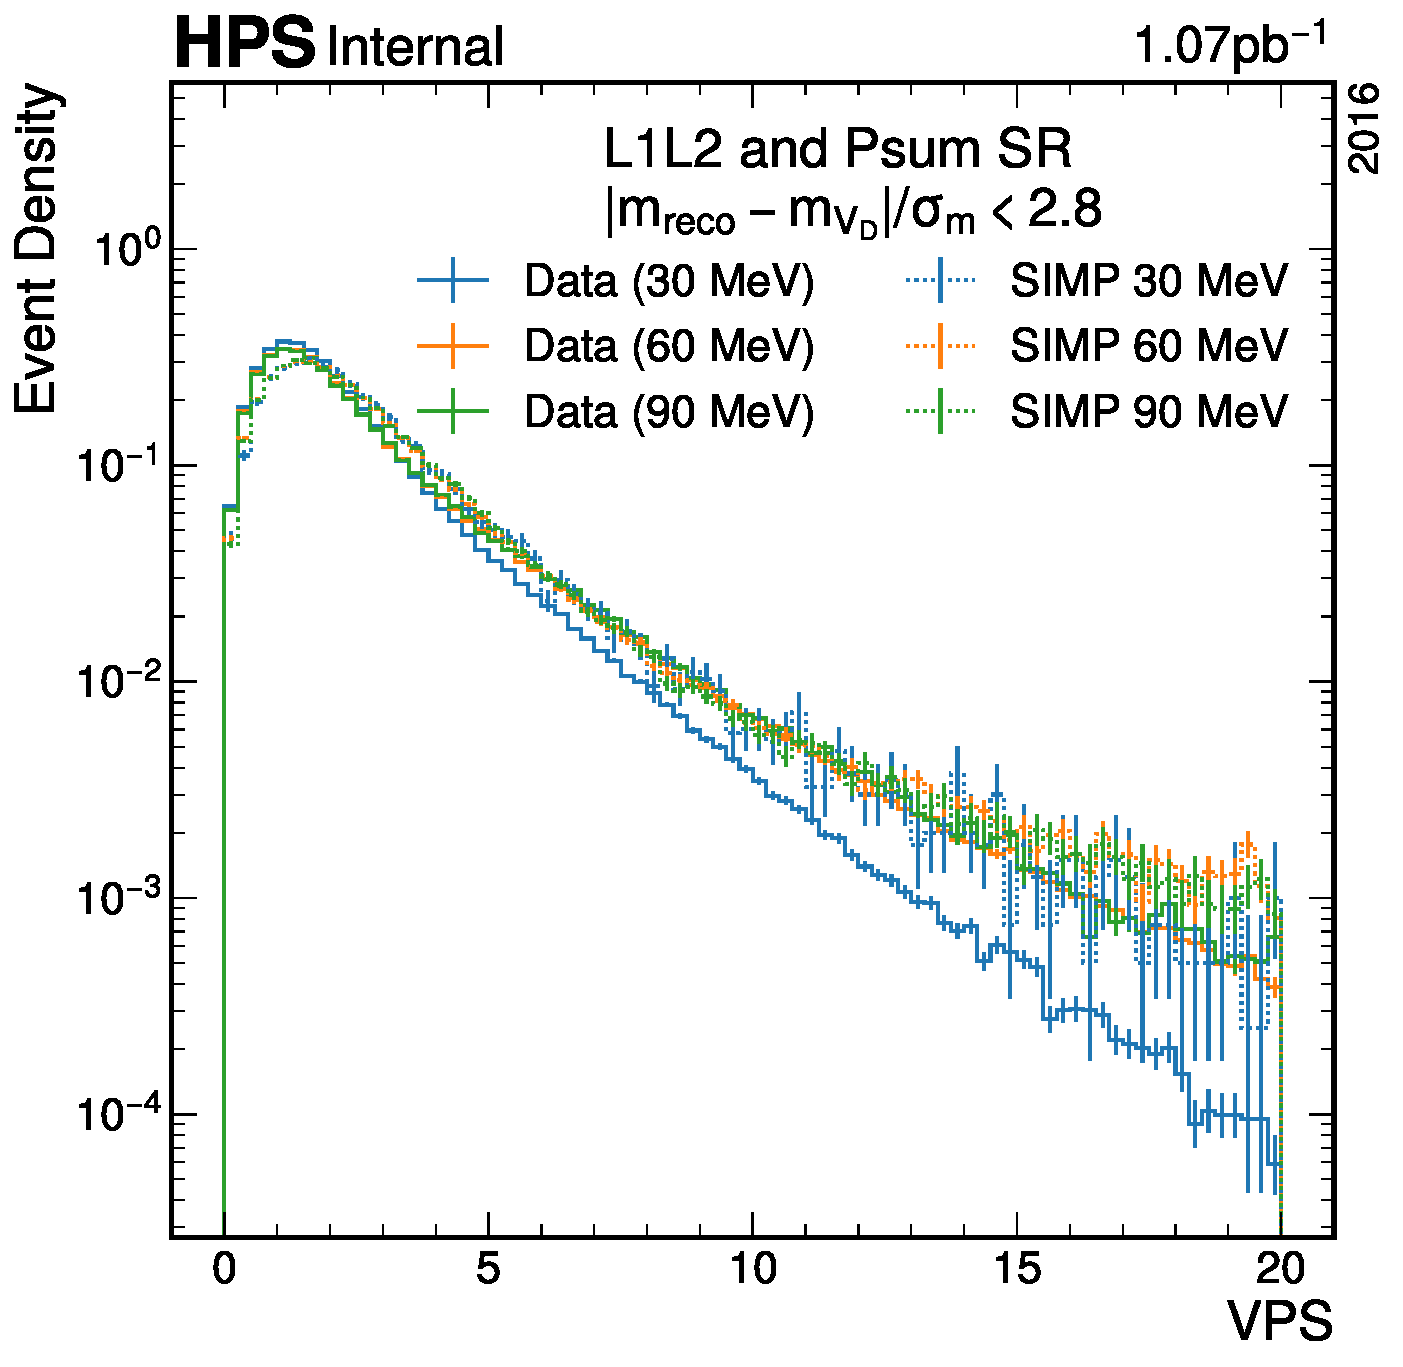
\includegraphics[width=\textwidth]{figures/hps/analysis/vtx_proj_sig-distribution.pdf}
    \caption{\ac{vps}}
    \label{fig:data-signal-comp:vps}
  \end{subfigure}
  ~
  \begin{subfigure}{0.30\textwidth}
    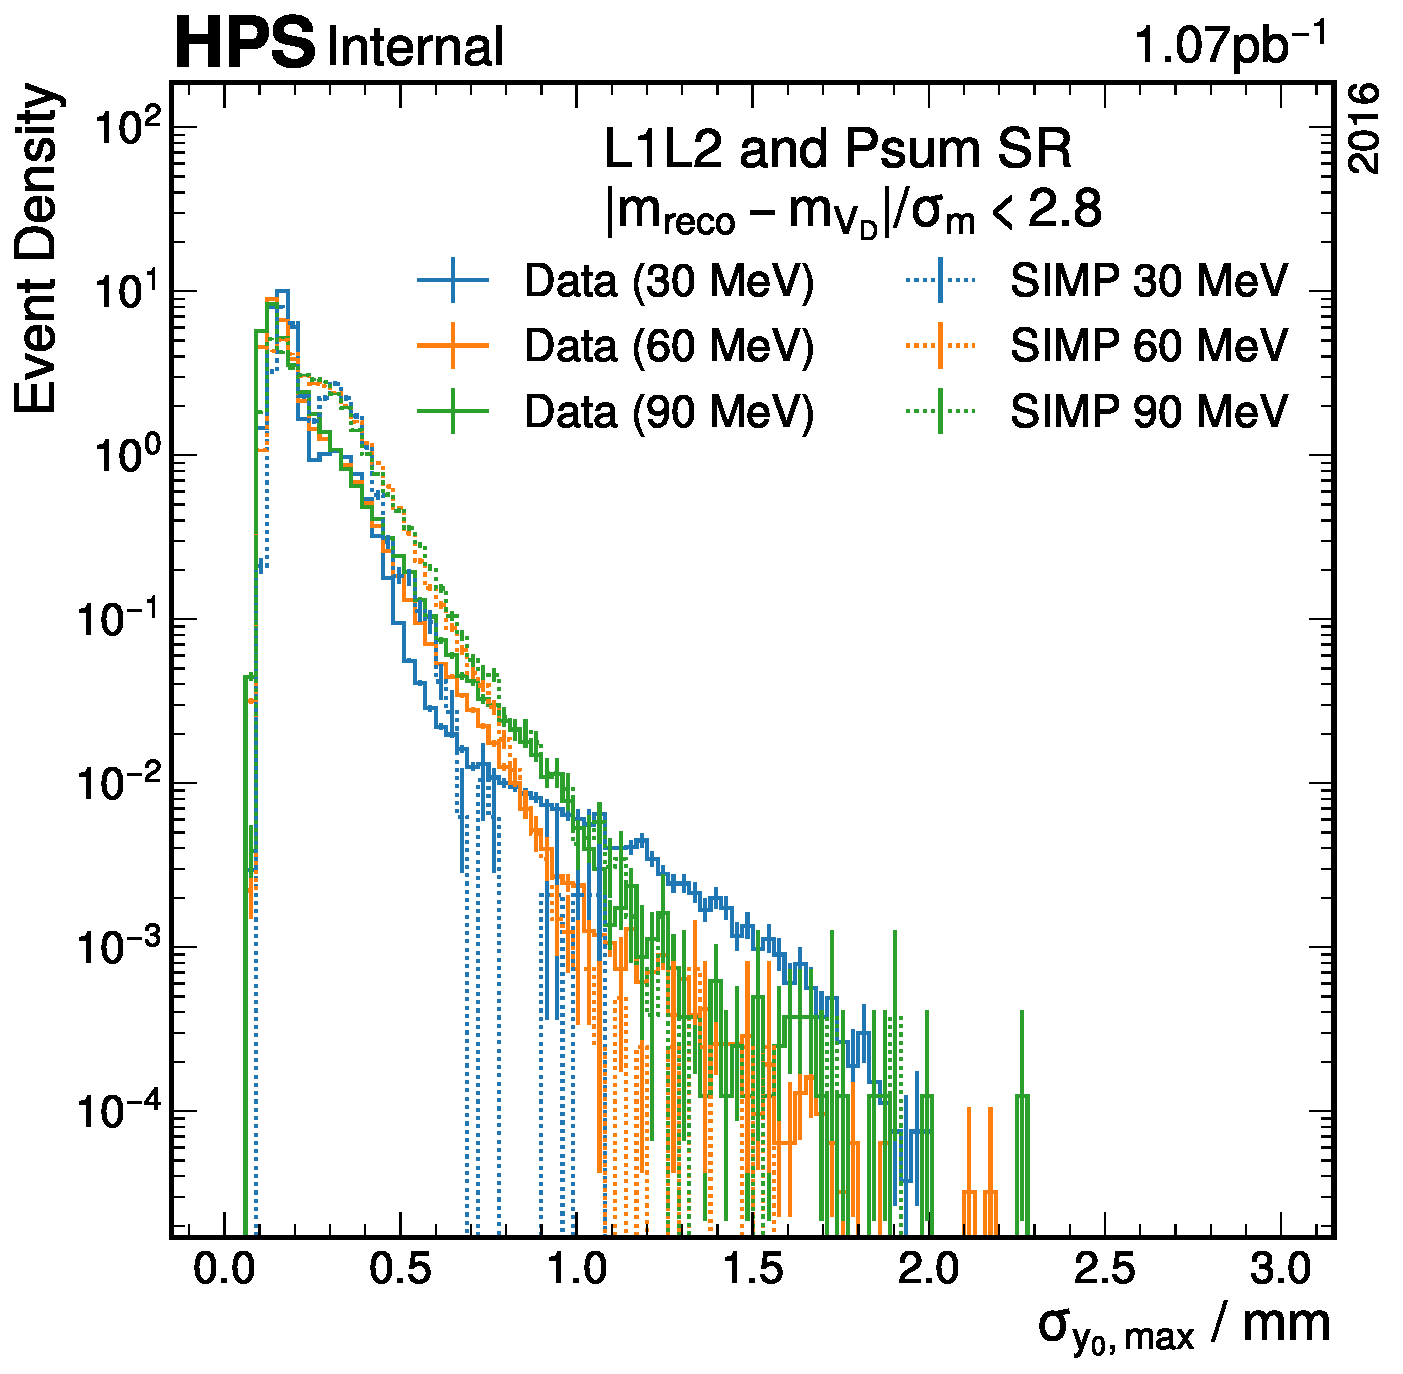
\includegraphics[width=\textwidth]{figures/hps/analysis/max_y0_err-distribution.pdf}
    \caption{\maxyzeroerr}
    \label{fig:data-signal-comp:max-y0-err}
  \end{subfigure}
  ~
  \begin{subfigure}{0.30\textwidth}
    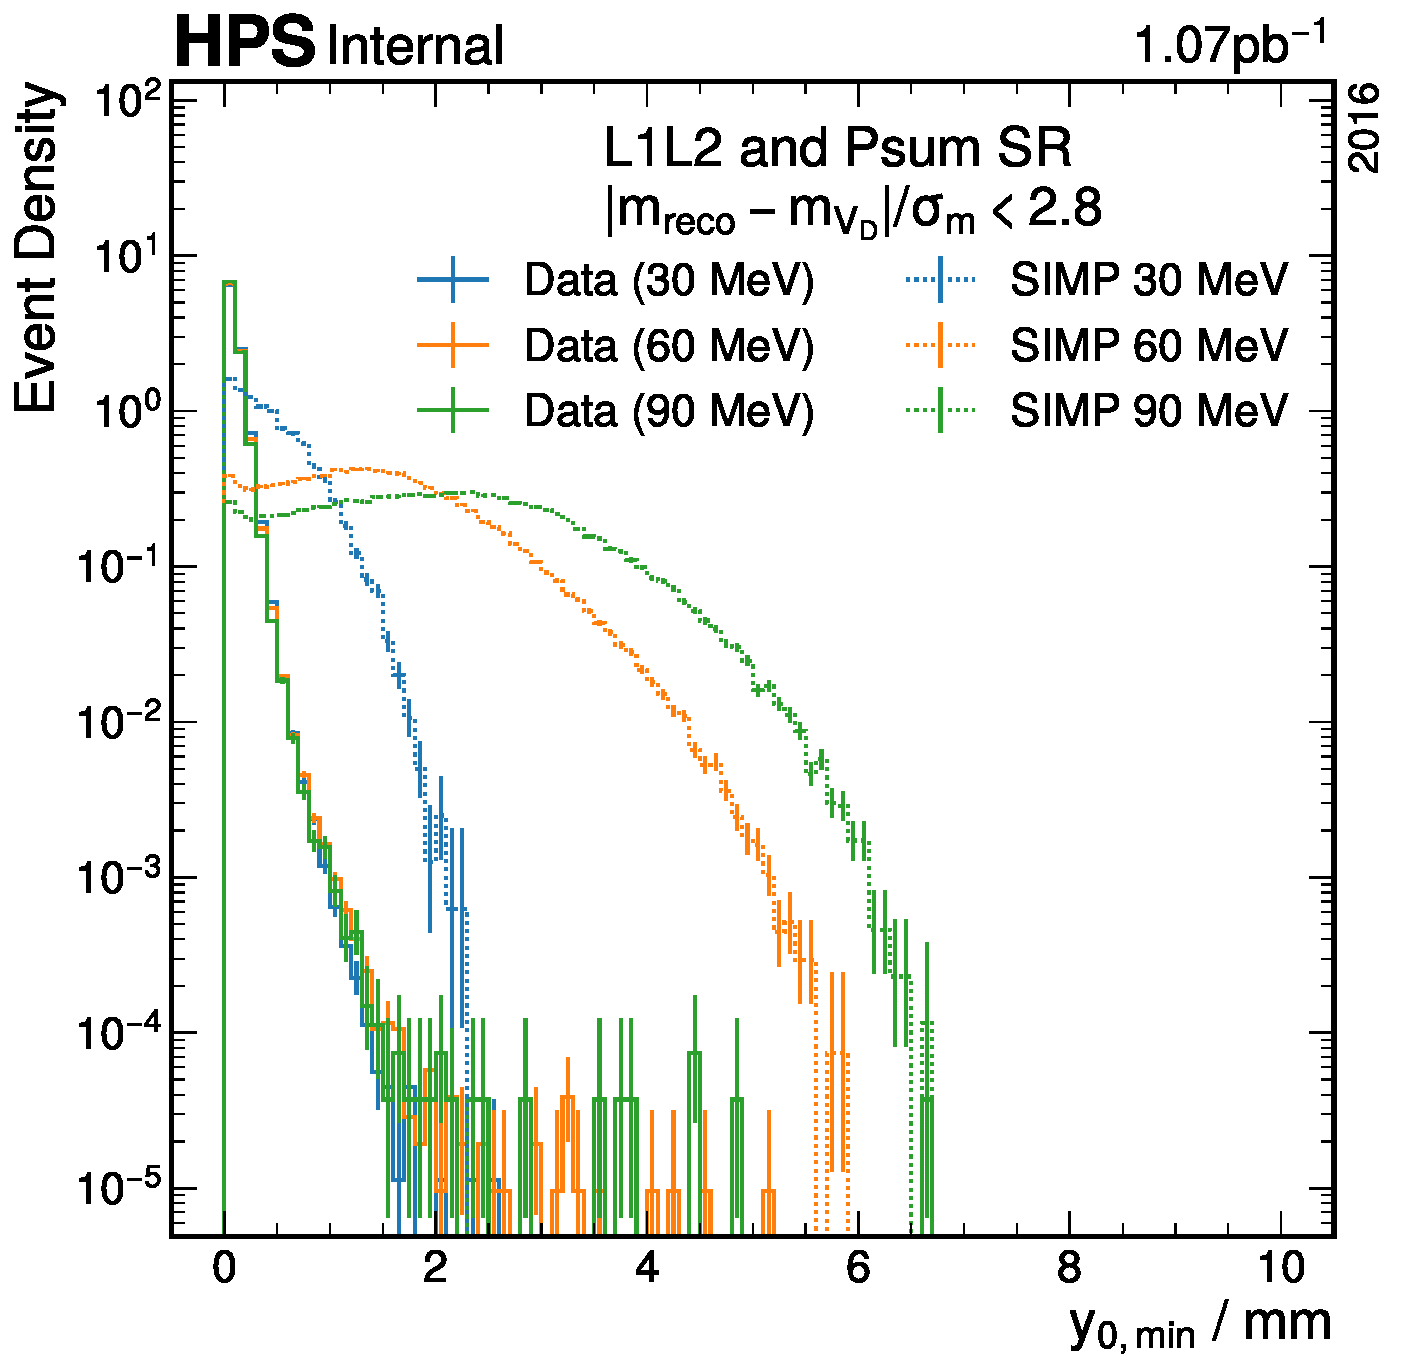
\includegraphics[width=\textwidth]{figures/hps/analysis/min_y0-distribution.pdf}
    \caption{\minyzero}
    \label{fig:data-signal-comp:min-y0}
  \end{subfigure}
  \caption{%
    Distributions of cut variables for a few example mass points.
    The vertices are required to be L1L2, have their momentum sum be within
    the signal region, and their invariant mass within the specified mass window.
  }
  \label{fig:data-signal-comp}
\end{figure}

Vertex $z$ is left for late-stage statistical analysis of the results
and - being highly correlated with \minyzero - is redundant with this variable.
